%Erzeuge mit pdflatex direkt pdfs statt dvi
\pdfoutput=1\relax
\pdfcompresslevel=9
%\pdfpagewidth=8.26in
%\pdfpageheight=11.69in

%&latex
% headsepline: Linie am oberen Blattrand unterhalb der Seitennummer
% bibtotoc: Aufnahme des Literaturverzeichnisses ins Inhaltsverzeichnis
\documentclass[a4paper,headsepline, bibtotoc]{scrreprt}
\usepackage[utf8]{inputenc}
\usepackage[T1]{fontenc}

% Einstellungen bez. des 'scrreprt'-Stils

% Caption Schriftstil und -Groesse
\renewcommand{\capfont}{\normalsize}
\renewcommand{\caplabelfont}{\normalsize\bfseries}

\typearea{15}  %Einstellung des Verhältnisses Größe des Textes zur Papiergröße

% Sprache
\usepackage[english]{babel}
\addto\extrasgerman{\renewcommand{\figurename}{Abb.}}
\addto\extrasgerman{\renewcommand{\tablename}{Tab.}}


% Bilder
\usepackage{epsfig,wrapfig}
\usepackage{graphicx}

% Bild und Tabellenunterschriften:
\usepackage{prettyref}
% für referenzen, z.B. label für section: \label{sec:abschnittslabel}verwenden
\newrefformat{eq}{\textup{(\ref{#1})}}
\newrefformat{cha}{Chapter~\ref{#1}}
\newrefformat{sec}{Section~\ref{#1}}
\newrefformat{app}{Appendix~\ref{#1}}
\newrefformat{tab}{Tab.~\ref{#1}}
\newrefformat{fig}{Fig.~\ref{#1}}
\newrefformat{no}{no.~\ref{#1}}
\newcommand\rf[1]{\prettyref{#1}}

% write 1st 2nd and 3rd.,.. with super and subscripts
\newcommand{\st}[0]{\textsuperscript{st} }
\newcommand{\nd}[0]{\textsuperscript{nd} }
\newcommand{\rd}[0]{\textsuperscript{rd} }

% kleine rechnungen für längen bei \setlength,\setcounter, \addtocounter \addtolength
\usepackage{calc}


% Mathematische Symbole
\usepackage{amsmath,amssymb}

% Macht alles ein wenig schöner
\usepackage{microtype}

% Tabellen
\usepackage{multicol}
\usepackage{longtable,lscape}
\usepackage{multirow}
\usepackage{tabularx}
\usepackage{array}
\usepackage{footmisc} % für Fussnoten in Tabellen,, verwendet den Befehl \mpfootnotemark

% Kopfzeilen
\usepackage{fancyhdr}
\pagestyle{plain}
\renewcommand{\chaptermark}[1]{\markboth{#1}{}}
\renewcommand{\sectionmark}[1]{\markboth{\thesection\ #1}{}}
\lhead[\fancyplain{}{\sl\leftmark}]%
      {\fancyplain{}{\sl\leftmark}}
\rhead[\fancyplain{}{\sl\thepage}]%
      {\fancyplain{}{\sl\thepage}}
\cfoot{}


% Listenerscheinung
\setlength{\itemsep}{0ex}
\setlength{\parsep}{0ex}
\setlength{\parskip}{2mm}
\setlength{\parindent}{0pt}                   % Einrueckung 1. Zeile eines Absatzes

%%%%%%%%%%%%%%%%%%%%%%%%%%%%%%%%%%%%%%%%%%%%%%%%%%%%%%%%%%%%%
%kompilieren: damits schneller geht, nur die kompilieren, die sich ändern!
%\includeonly{}
%%%%%%%%%%%%%%%%%%%%%%%%%%%%%%%%%%%%%%%%%%%%%%%%%%%%%%%%%%%%%
\begin{document}
\sloppy

% Titelseite
\begin{titlepage}

% Titelseite
\title{HDF5 Mesh Documentation}

\author{\\
          Florian Hindenlang, Thomas Bolemann }


\date{last modified: \today}
\publishers{Institut für Aerodynamik und Gasdynamik, \\
            Universität Stuttgart}



\end{titlepage}
% Seitennumerierung bis zum Beginn der Einleitung auf kleine roemische Zahlen setzen
\pagenumbering{roman}
\maketitle

% Inhaltsverzeichnis
\addcontentsline{toc}{chapter}{Table of Contents}
\tableofcontents

\pagestyle{plain}
\renewcommand{\chaptermark}[1]{\markboth{#1}{}}
\renewcommand{\sectionmark}[1]{\markboth{\thesection\ #1}{}}
\lhead[\fancyplain{}{\sl\leftmark}]%
      {\fancyplain{}{\sl\leftmark}}
\rhead[\fancyplain{}{\sl\thepage}]%
      {\fancyplain{}{\sl\thepage}}
\cfoot{}

% Seitennumerierung ab der folgenden Einleitung auf arabische Zahlen setzen
\pagenumbering{arabic}


%Text
\newpage
\chapter{UNSTRUCTURED HOPR HDF5 MESHFORMA}

Main idea: save all side and node informations more than once, but always in a package per element. In parallel, this would allow to read in a block of element, side and node information The only array which is not read in blocks is the Node coordinates.\\
Indexing starts at 1! (Fortran Style)

\section{File}
\subsection{Mesh Attributes}

These attributes are defined globally for the whole mesh.

\begin{table}[h!]
\centering
\begin{tabularx}{1.0\textwidth}{|l|l|X|} \hline
Attribute     & Value     & Description \\ \hline
BoundaryOrder & 1\ldots $N_g$ & Order of geometry approximation. Needed to determine the number of internal nodes of curved volumes. \\
CurvedFound   & 0 / 1     & 0 = no curved volumes, 1 = curved volumes \\\hline
\end{tabularx}
\caption{Types of Elements}
\end{table}

\subsection{Group Members}
\begin{table}[h!]
\centering
\begin{tabularx}{1.0\textwidth}{|l|X|l|} \hline
Property      & Description                                             & Type/Size          \\ \hline
BCNames       & user-defined boundary condition names                   & String/(nBCs,1)     \\
BCType        & four digit boundary condition code  & Integer/(nBCs,4)   \\ 
ElemBarycenters   & Barycenter location of each element  & Real/(nElems,3)  \\
ElemCounter   & mesh statistics (no. of elements of each element type)  & Integer/(nTypes,2)  \\
ElemInfo      & Element Data                                             & Integer/(nElems,6)  \\
ElemWeight    & Element Weights                                         & Real/(nElems,1)    \\ 
NodeCoords    & Node Coordinates                                        & Real/(nNodes,3)  \\
NodeInfo      & List of Node IDs for each element / side                & Integer/(:,1)       \\ 
SideInfo      & Side Data / Connectivity                                & Integer/(:,4)       \\ \hline
\end{tabularx}
\caption{Types of Elements}
\end{table}

Einfuegen eines schoenen bildes mit 108 und 208 Element
\section{Definitions}
\subsection{Element Information}

\begin{table}[h!]
\begin{tabularx}{1.0\textwidth}{lX}
Name in HDF5: & \textbf{ElemInfo} \\
Type:         & INTEGER, Size: Array(nElems,6) \\
Description:  & Array containing elements, one element per row, row number is elemID. \\
\end{tabularx}
\end{table}

\begin{table}[h!]
\centering
\begin{tabular}{|l|l|l|l|l|l|l|} \hline
  & Element Type & ZoneNr & firstIndSIDE & lastIndSIDE & firstindNODE & lastIndNODE \\ \hline
1 & 118 & 1 & 0 & 6 & 0 & 14 \\ \hline
2 & 118 & 1 & 6 & 12 & 14 & 28 \\ \hline
\end{tabular}
\caption{Example of \textbf{ElemInfo} array for two elements}
\end{table}

\begin{table}[h!]
\centering
\begin{tabularx}{0.4\textwidth}{|X|l|} \hline
ElementType        &Index\\ \hline
Hexaeder, linear   & 108  \\
Hexaeder, bilinear   & 118 \\
Hexaeder, nonlinear  & 208 \\ \hline
\end{tabularx}
\caption{Definition of Element Types}
\end{table}
The number of element corner nodes is known from the element type, whereas nonlinear means that the element has curved sides. These curved sides are represented by interpolation nodes, and the number of interpolation nodes depends on the boundary order.

\emph{firstIndNode/lastIndNode}: Instead of storing the node information directly inside the element, each element has a range of nodes in the \textbf{NodeInfo} array with unique NodeIDs. The range is unique to each element.

\emph{firstSideInd/lastSideInd}: The side information is handled the same way. A range of sides in the \textbf{SideInfo} is defined for the element.

\emph{firstIndSide/lastIndSide}: first index -1 / last index in \textbf{SideInfo} array for this element, size = last - first \\
\emph{firstIndNode/lastIndNODE}: first index -1 / last index in \textbf{NodeInfo} array for this element with this array bounds for reading SIDE and NODE arrays are clear

The data is always stored elementwise, which results in storing it multiple times. However, this way, each processor has a defined, non overlapping, range of side /node information, where it can perform IO operations, minimizing the need of communication between processors. 

Zone beschreibung am CGNS Zones z.B.

\newpage

\subsection{Side Information}

\begin{table}[h!]
\begin{tabularx}{1.0\textwidth}{lX}
Name in HDF5: & \textbf{SideInfo} \\
Type:         & INTEGER, Size: Array(ElemInfo(nElems,lastSideInd)-ElemInfo(1,firstSideInd),4) \\
Description:  & Side array, all information of one element is a package innersides will be referred twice. \\
\end{tabularx}
\end{table}

\begin{table}[h!]
\centering
\begin{tabular}{|l|l|l|l|l|l|}
\hline
 & SideType & SideID & nbElemID & BCID & in \textbf{ElemInfo}\\ \hline
1 & 5 & 1 & 0 & 5 &  firstIndSIDE+1 \\ 
2 & 5 & 2 & 0 & 3 &  \\ 
3 & 5 & 3 & 2 & 0 &  \\ 
4 & 5 & 4 & 0 & 4 &  \\ 
5 & 5 & 5 & 0 & 1 &  \\ 
6 & 5 & 6 & 0 & 6 &  lastIndSIDE \\ \hline
7 & 5 & 7 & 0 & 5 &  firstIndSIDE+1 \\ 
8 & 5 & 8 & 0 & 3 &  \\ 
9 & 5 & 9 & 0 & 2 &  \\ 
10 & 5 & 10 & 0 & 4 &  \\ 
11 & 5 & -3 & 1 & 0 &  \\ 
12 & 5 & 11 & 0 & 6 & lastIndSIDE \\ \hline
\end{tabular}
\caption{Example \textbf{SideInfo} array}
\end{table}

\begin{table}[h!]
\centering
\begin{tabularx}{0.5\textwidth}{|X|l|} \hline
SideType         &Index   \\ \hline
line, linear/curved & 1/2 \\
 Quad, bilinear     & 5   \\
 Quad, nonlinear    & 7   \\ \hline
\end{tabularx}

\caption{Definition of Element Types}
\end{table}
\begin{table}[h!]
\begin{tabularx}{1.0\textwidth}{lX}
\emph{SideID}:          & unique side identifier, can be directly used as MPItag, negative if side is not oriented \\
\emph{SideType}:        & From SideType, the number of corner nodes is known (triangle/quadrangle), and if the side is curved. The number of nodes for curved triangles: $N_g(N_g+1)/2$ and quadrangles: $N_g^2$. \\
\emph{neighborElemID}:  & ID of neighbor element. This helps to quickly build up element connections, for local as well as inter-processor element connections. \\
\emph{BCID}:            & index in BCName / BCType array. If periodic, nbElemID is given, SideID is the same, but other nodes!!! 
\end{tabularx}
\end{table}

The BCID entries refer to a list of user-defined boundary-conditions, stored in the array \textbf{BCNames}. 

\newpage

\subsection{Node Information}

\begin{table}[h!]
\begin{tabularx}{1.0\textwidth}{lX}
Name in HDF5: & \textbf{NodeInfo}\\
Type:         & INTEGER, Size: Array(ElemInfo(nElems,lastNodeInd)-ElemInfo(1,firstNodeInd),1) \\
Description:  & One dimensional array of node IDs, again one package for one element.   \\
\end{tabularx}
\end{table}

\begin{table}[h!]
\centering
\begin{tabular}{|l|c||l|l|} \hline
  & nodeID & &\\ \hline
1 & 1 &  first elem corner node&  firstIndNODE+1 \\
2 & 2 &  &  \\ 
3 & 4 &  &  \\ 
4 & 3 &  &  \\ 
5 & 5 &  &  \\ 
6 & 6 &  &  \\ 
7 & 8 & &  \\ 
8 & 7 &   last elem corner node  &  \\ \hline
9 & 1 &  &  \\ \hline
10 & 1 &  &  \\ \hline
11 & 2 &  &  \\ \hline
12 & 4 &  &  \\ \hline
13 & 1 &  &  \\ \hline
14 & 5 &  &  \\ \hline
15 & 9 &  first elem corner node &  \\
16 & 10 &  &  \\ 
17 & 12 &  &  \\ 
18 & 11 &  &  \\
19 & 13 &  &  \\ 
20 & 14 &  &  \\
21 & 16 &  &  \\ 
22 & 15 &  last  elem corner node &  \\  \hline
23 & 9 &  &  \\ \hline
24 & 9 &  &  \\ \hline
25 & 10 &  &  \\ \hline
26 & 12 &  &  \\ \hline
27 & 9 &  &  \\ \hline
28 & 13 &  &  lastIndNODE \\ \hline
\end{tabular}
\caption{Node information for a linear tetrahedron}
\end{table}
The node information is packed element-wise. The element corner nodes are defined first, given by the first four entries in the example above. The following nodeIDs define the the first oriented nodes of each side of the element. The oriented node is needed, since the neighbor side is not known a priori. The sideID from \textbf{SideInfo} array is negative for non-oriented sides. If the side is a master the oriented node is the nodeID of the first side node. If the side is a slave (sideID negative) the oriented node is the nodeID of the side node corresponding to the master first node.
\newpage

\begin{figure}
\centering
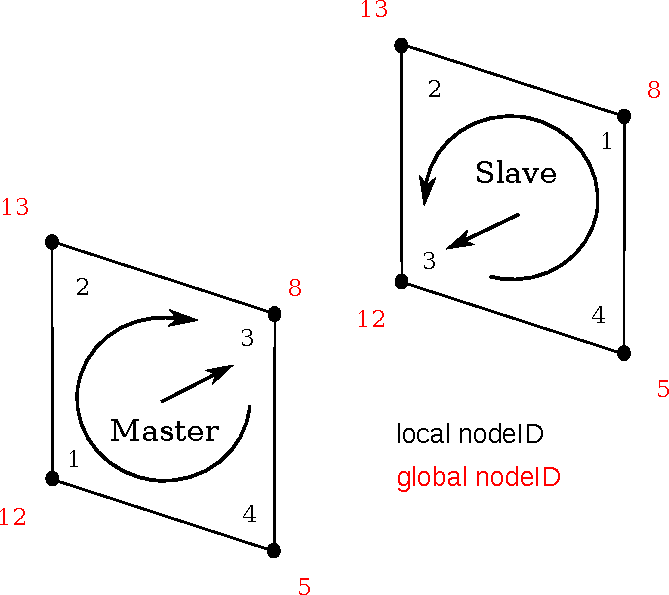
\includegraphics[width=0.5\textwidth]{masterslave.pdf}
\caption{Node orientation for master and slave node}
\label{labelname}
\end{figure}

Curved elements require the definition of additional interpolation points:
\begin{table}[h!]
\centering
\begin{tabular}{|l|c||l|l|} \hline
   & nodeID & &\\ \hline
1 & 1 & first elem corner node & firstIndNODE+1 \\ 
2 & 3 &  &  \\ 
3 & 9 &  &  \\ 
4 & 7 &  &  \\
5 & 19 &  &  \\ 
6 & 21 &  &  \\ 
7 & 27 &  &  \\ 
8 & 25 & last elem corner node &  \\ \hline
9 & 1 & first curved nodeID &  \\
10 & 2 &  &  \\ 
11 & 3 &  &  \\ 
12 & 4 &  &  \\ 
13 & 5 &  &  \\ 
14 & 6 &  &  \\ 
15 & 7 &  &  \\ 
16 & 8 &  &  \\ 
\ldots & \ldots & last curved nodeID &  \\ \hline
\end{tabular}
\caption{Node information for a hexa}
\end{table}

The ordering of the interpolation nodes is then defined by sets as depicted in \prettyref{fig:quad} and \prettyref{fig:tri}, where each set represents the additional points required by a certain boundary order. The number of points in the $i-$th row is $2i+1$ for quadrangular and $i$ for triangular sides.  

\newpage

\subsection{Node Coordinates}

\begin{table}[h!]
\begin{tabularx}{1.0\textwidth}{lX}
Name in HDF5: & \textbf{NodeCoords}\\
Type:         & REAL \quad Size: Array(1:nNodes,nDim) \\
Description:  & The coordinates of nodes, will be the only array which cannot be accessed in packages, since each unique node is normally used more that once. For parallel IO, each processor has to extract the list of nodeIDs from the information in \textbf{NodeInfo} array. \\
\end{tabularx}
\end{table}


\newpage

\subsection{Boundary Conditions}

\begin{table}[h!]
\begin{tabularx}{1.0\textwidth}{lX}
Name in HDF5: & \textbf{BCNames} \\
Type:         & STRING, Size: Array(nBCs,1)  \\
Description:  & User-defined array of boundary-conditions. \\
\end{tabularx}
\end{table}

The boundary conditions are completely defined by the user. Each BCID from the sideInfo array has to be specified in the \textbf{BCNames} array first.

\begin{table}[h!]
\centering
\begin{tabular}{|l|l|} \hline
Ind & Boundary Conditions Name: \\ \hline
1   &  PeriodicPlus\\
2   &  PeriodicMinus\\
3   &  Inflow\\
4   &  Outflow\\
5   &  Wall\\
6   &  wallcurved\\ \hline
\end{tabular}
\caption{Example for boundary conditions}
\end{table}


\section{Mortars}

\subsection{Element Information}

\begin{table}[h!]
\centering
\begin{tabular}{|l|l|l|l|l|l|l|} \hline
  & Element Type & ZoneNr & firstIndSIDE & lastIndSIDE & firstindNODE & lastIndNODE \\ \hline
1 & 118 & 0 & 0 & 6 & 0 & 14 \\ \hline
2 & 118 & 0 & 6 & 12 & 14 & 28 \\ \hline
3 & 118 & 0 & 12 & 18 & 28 & 42 \\ \hline
4 & 118 & 0 & 18 & 24 & 42 & 56 \\ \hline
5 & 118 & 0 & 24 & 30 & 56 & 70 \\ \hline
6 & 118 & 0 & 30 & 36 & 70 & 84 \\ \hline
7 & 118 & 0 & 36 & 42 & 84 & 98 \\ \hline
8 & 118 & 0 & 42 & 48 & 98 & 112 \\ \hline
9 & 118 & 0 & 48 & 58 & 112 & 126 \\ \hline
\end{tabular}
\caption{Example of \textbf{ElemInfo} array for two trees: one tree is refined (level one)}
\end{table}

\newpage

\subsection{Side Information}

\begin{table}[h!]
\centering
\begin{tabular}{|l|l|l|l|l|l|}
\hline
 & SideType & SideID & nbElemID & BCID & in \textbf{ElemInfo}\\ \hline
1 & 5 & 37 & 0 & 5 &  \\ \hline
2 & 5 & 38 & 0 & 3 &  \\ \hline
3 & 5 & 39 & 0 & 2 &  \\ \hline
4 & 5 & 40 & 0 & 4 &  \\ \hline
5 & 5 & 41 & -1 & 0 &  side with connected mortars \\ \hline
6 & 5 & 9 & 2 & 0 &  mortar sides\\ \hline
7 & 5 & 18 & 4 & 0 &  ...\\ \hline
8 & 5 & 27 & 6 & 0 &  ...\\ \hline
9 & 5 & 34 & 8 & 0 &  ...\\ \hline
10 & 5 & 42 & 0 & 6 &  \\ \hline
\end{tabular}
\caption{Example \textbf{SideInfo} array with mortars}
\end{table}


\begin{figure}[h!]
\centering
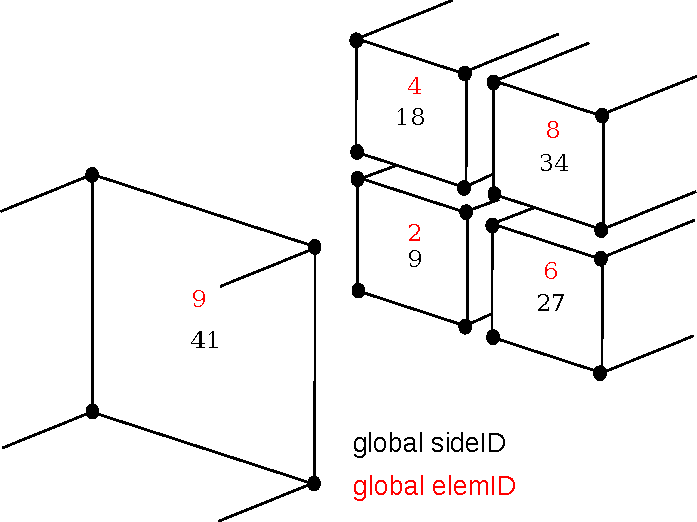
\includegraphics[width=0.5\textwidth]{mortar.pdf}
\caption{Mortar side and elements}
\label{labelname}
\end{figure}




% \subsection{Hanging Faces}
% 
% \begin{table}[h!]
% \begin{tabularx}{1.0\textwidth}{lX}
% Name in HALO: & HAND (?) \\
% Name in HDF5: & --- (?)  \\
% Type:     & INTEGER \quad Array(nHangingFaces,3,nDim-1) \\
% Description:  &  For hanging nodes/faces, additional parameter informations have to be saved, since the original side will remain unique. Hanging sides will only be allowed for binary splits, so that we could save only integer fractions.  \\           
%               & t0: corner coordinates in parameter space \\
%               & deltat: extend of side in paramter space \\  
%               & exp: $2^{exp}$, which is the biggest denominator (number of splits) the coordinates of the points will then be
%             $t0(1)/2^{exp},t0(2)/2^{exp}) , ( (t0(1)+dt(1)/2^{exp},t0(2)/2^{exp})$ ... or save as 2xnDim-1 REAL \\
% 
% \end{tabularx}
% \end{table}
% 
% If no hanging side, no entries.  













% \subsection{Zonal Data Input}
% A mesh can be subdivided in zones. Zonal variables can be defined
% for each zone separately or in groups. An example is shown below,
% where one viscosity is first assigned to all 3 zones, and then
% changed for zone 1 and 3.
% \begin{center}
% \begin{minipage}{0.3\textwidth}
% \begin{verbatim}
% Mesh%nZones=3
% ...
% DISC%mu=0.01
% DISC%mu=0.05 #1 #3
% \end{verbatim}
% \end{minipage}
% \end{center}
% \section{List of Variables}
% All variables are listed in \rf{tab:inifile}.
% \begin{landscape}
% 
%   % for the flowchart, use boxes and arrows, predefined here:
%   %--------------------------------------------------------------------------%
%   \newcounter{numb}
%   \newenvironment{nb}{\refstepcounter{numb}\thenumb }{}
%   \newlength\nbrs \settowidth\nbrs{999}
%   \newlength\tabs \setlength\tabs{8em}
%   \newlength\dsc  \setlength\dsc{15em}
% 
%  % first level indent
%   \newcommand\varline[9]{
%            #1
%            & \ttfamily #2
%            & \begin{tabular}[t]{m{\tabs}m{\tabs}m{\tabs}l}
%               \rule[-1ex]{0ex}{4ex} \centering #3 & \centering #5 & \centering #7 &\\ \hline
%               \rule[-1ex]{0ex}{4ex} \centering #4 & \centering #6 & \centering #8 &
%              \end{tabular}
%            & #9 & \\ \cline{2-5}}
%   \newcommand\levela{$\Rightarrow$\hspace{0.5em}}
%   \newcommand\levelb{\hspace{1em}$\Rightarrow$\hspace{0.5em}}
%     %--------------------------------------------------------------------------%
%   \scriptsize
%     %---------------------------------------------------------------------------------------------
%     \setlength\extrarowheight{2pt}
%     \begin{longtable}[c]{m{\nbrs}lm{3.5\tabs}m{\dsc}l}
%     %---------------------------------------------------------------------------------------------
%     % arguments for longtable
%         \caption{inputfile variables  \label{tab:inifile}} \tabularnewline
%         \hline
%         %title
%         \bfseries No.
%            &  \bfseries\centering Variable name
%                & \begin{tabular}[t]{m{\tabs}m{\tabs}m{\tabs}l}
%                    \bfseries \rule[-1ex]{0ex}{4ex} \centering Category
%                     &  \bfseries\centering Type
%                       & \bfseries\centering Zonal/Global  & \\ \hline
%                   \bfseries\centering \rule[-1ex]{0ex}{4ex} Compilerflag
%                     & \bfseries\centering  Array Dim.
%                       & \bfseries\centering default value &
%                  \end{tabular}
%                      & \bfseries\centering description  &   \\ \hline \hline
%     \endfirsthead
%     % header on the next pages
%         \caption[]{inputfile variables \footnotesize\sl (continued from previous page)}\tabularnewline
%         \hline
%         %title
%         \bfseries No.
%            &  \bfseries\centering Variable name
%                & \begin{tabular}[t]{m{\tabs}m{\tabs}m{\tabs}l}
%                    \bfseries \rule[-1ex]{0ex}{4ex} \centering Category
%                     &  \bfseries\centering Type
%                       & \bfseries\centering Zonal/Global  & \\ \hline
%                   \bfseries\centering \rule[-1ex]{0ex}{4ex} Compilerflag
%                     & \bfseries\centering  Array Dim.
%                       & \bfseries\centering default value &
%                  \end{tabular}
%                      & \bfseries\centering description  &   \\ \hline \hline
%      \endhead
%     % footer on the next pages
%         \multicolumn{4}{r}{\footnotesize\sl continued on next page}\tabularnewline
%     \endfoot
% %         \hline
% %         \multicolumn{6}{r}{\scriptsize *Anmerkung}\tabularnewline
%     \endlastfoot
%     %---------------------------------------------------------------------------------------------
%     \varline{\nb }% number and \label{no:  } if needed
%         {DISC\%c\_corr  } %variable name
%         {MHD}{DIVCORR}{REAL}{1}{G}{1.0} % Category, Compiler, Type, Zonal, Default
%         {max. divergence correction speed in times of the fastest system speed}
%     %---------------------------------------------------------------------------------------------
%     \varline{\nb }% number and \label{no:  } if needed
%         {MESH\%nZones}
%         {MESH}{-}{INTEGER}{1}{G}{MANDATORY}
%         {number of zones = number of carteisan meshes / all zones in mesh files}
%     %---------------------------------------------------------------------------------------------
%     \varline{\nb }% number and \label{no:  } if needed
%         {DISC\%TimeOrder}
%         {SOLVER}{-}{INTEGER}{1}{ZONAL/ORDER}{0}
%         {Specifies the order of the STE-DG scheme in time. For a given order.}
%     %---------------------------------------------------------------------------------------------
%     \varline{\nb }% number and \label{no:  } if needed
%         {MESH\%minorder}
%         {ADAPTIVITY}{-}{INTEGER}{1}{G}{1}
%         {minimum order for p-recoarse  during adaptivity, ???save for max 8 zones?}
%     %---------------------------------------------------------------------------------------------
%     \varline{\nb }% number and \label{no:  } if needed
%         {MESH\%maxorder}
%         {ADAPTIVITY}{-}{INTEGER}{1}{G}{6}
%         {maximum order, limit for adaption}
%     %---------------------------------------------------------------------------------------------
%         \varline{\nb }% number and \label{no:  } if needed
%             {\levela  MESH\%ScaleSepOrder}
%             {???}{VMS}{INTEGER}{1}{ZONAL}{2}
%             {???}
%     %---------------------------------------------------------------------------------------------
%     \varline{\nb }% number and \label{no:  } if needed
%         {DISC\%IPmode2d}
%         {SOLVER}{-}{INTEGER}{1}{G}{1}
%         {increase the number of interpolation points in 2D elements}
%     %---------------------------------------------------------------------------------------------
%     \varline{\nb }% number and \label{no:  } if needed
%         {DISC\%IPmode3d}
%         {SOLVER}{-}{INTEGER}{1}{G}{2}
%         {increase the number of interpolation points in 3D elements}
%     %---------------------------------------------------------------------------------------------
%     \varline{\nb }% number and \label{no:  } if needed
%         {DISC\%IPsuperorder}
%         {SOLVER}{-}{INTEGER}{1}{G}{0}
%         {increase the interpolation order (number of points) at the boundaries.}
%     %---------------------------------------------------------------------------------------------
%     \varline{\nb }% number and \label{no:  } if needed
%         {DISC\%SpaceQuandt}
%         {MESH}{-}{REAL}{1}{G}{0.1}
%         {Characteristic length in the mesh. Used as tolerance in general and for connectivity.}
%     %---------------------------------------------------------------------------------------------
%     \varline{\nb }% number and \label{no:  } if needed
%         {MESH\%projectname}
%         {OUTPUT}{-}{STRING}{1}{G}{MANDATORY}
%         {project name, used for all outpur files}
%     %---------------------------------------------------------------------------------------------
%     \varline{\nb }% number and \label{no:  } if needed
%         {DISC\%visuMode}
%         {RESTART / VISU}{-}{INTEGER}{1}{G}{1}
%         {\mbox{1: compute and visualize,   \hspace{4cm}}
%          \mbox{2: compute only,            \hspace{4cm}}
%          \mbox{3: visualize form database  \hspace{4cm}}}
%     %---------------------------------------------------------------------------------------------
%     \varline{\nb }% number and \label{no:  } if needed
%         {DISC\%VisuGradVelocity}
%         {VISU}{-}{LOGICAL}{1}{G}{F}
%         {add velocity gradient to visulaized variables (*visu*.cgns)}
%     %---------------------------------------------------------------------------------------------
%     \varline{\nb }% number and \label{no:  } if needed
%         {DISC\%visuLambda2}
%         {VISU}{-}{LOGICAL}{1}{G}{F}
%         {visualize lambda2 criterion (vorticity)}
%     %---------------------------------------------------------------------------------------------
%     \varline{\nb }% number and \label{no:  } if needed
%         {DISC\%CalcBodyForces}
%         {POSTPROC}{-}{LOGICAL}{1}{G}{F}
%         {Calculate body forces and aerodynamic Coefficients ($c_a$, $c_w$ and $c_m$),
%          on boundaries:
%          \mbox{3 (BCWallViscousHeatFlux, BCWallViscous)},
%          \mbox{4 (BCWallViscousIsothermal, BCWall)} and \mbox{9 (BCWallInviscid)}.}
%     %---------------------------------------------------------------------------------------------
%     \varline{\nb }% number and \label{no:  } if needed
%         {DISC\%BodyForceS}
%         {POSTPROC}{-}{REAL}{1}{G}{1.0}
%         {Surface area for exact computations of aerodynamic Coefficients ($c_a$, $c_w$ and $c_m$),
%          on boundaries.}
%     %---------------------------------------------------------------------------------------------
%     \varline{\nb }% number and \label{no:  } if needed
%         {DISC\%CalcResiduum}
%         {POSTPROC}{ADIGMA}{LOGICAL}{1}{G}{F}
%         {Calculate residuum.}
%     %---------------------------------------------------------------------------------------------
%     \varline{\nb }% number and \label{no:  } if needed
%         {DISC\%reDelaunay}
%         {???}{???}{LOGICAL}{1}{G}{F}
%         {???.}
%     %---------------------------------------------------------------------------------------------
%     \varline{\nb }% number and \label{no:  } if needed
%         {MESH\%runterRamp}
%         {INITIALIZE}{-}{LOGICAL}{1}{G}{F}
%         {Ramp initial velocities of boundary elements from zero to initial values}
%     %---------------------------------------------------------------------------------------------
%     \varline{\nb }% number and \label{no:  } if needed
%         {DISC\%forceOneProc}
%         {MPI}{-}{LOGICAL}{1}{G}{F}
%         {force to do the initialization (fillMesh and co) on one processor}
%     %---------------------------------------------------------------------------------------------
%     \varline{\nb \label{no:meanfield} }% number and \label{no:  } if needed
%         {MESH\%getMeanField}
%         {INITIALIZE}{APE}{LOGICAL}{1}{G}{F}
%         {switch to specify the mean value source (file or ini) for APE}
%     %---------------------------------------------------------------------------------------------
%         \varline{\nb }% number and \label{no:  } if needed
%             {\levela MESH\%MeanFieldFile}
%             {INITIALIZE}{APE}{STRING}{1}{G}{mandatory if \rf{no:meanfield} T}
%             {file name of mean Field data file containing background field mean values for APE}
%     %---------------------------------------------------------------------------------------------
%     \varline{\nb \label{no:limitertype}}% number and \label{no:  } if needed
%         {DISC\%limiterType}
%         {LIMITER}{NS / MHD}{INTEGER}{1}{G}{0}
%         {\mbox{0:= no limiter;                           \hspace{4cm}}
%          \mbox{1:= mu limiter;                           \hspace{4cm}}
%          \mbox{2:= Persson limiter;                      \hspace{4cm}}
%          \mbox{4:= modified Persson limiter;             \hspace{4cm}}
%          \mbox{5:=combined Jameson/mesh-Reynolds limiter;\hspace{4cm}}}
%     %---------------------------------------------------------------------------------------------
%         \varline{\nb }% number and \label{no:  } if needed
%             {\levela DISC\%epsilon}
%             {SOLVER}{NS / MHD}{REAL}{1}{G}{0.0, if \rf{no:limitertype}$>0$}
%             {!! obsolete !!}
%     %---------------------------------------------------------------------------------------------
%         \varline{\nb }% number and \label{no:  } if needed
%             {\levela DISC\%D0}
%             {LIMITER}{NS / MHD}{REAL}{1}{G}
%             {0.0, if \rf{no:limitertype} $>0$}
%             {Scaling/tuning parameter for the limiter's viscosity.}
%     %---------------------------------------------------------------------------------------------
%     \varline{\nb \label{no:nvv}}% number and \label{no:  } if needed
%         {MESH\%nVV}
%         {MESH}{-}{INTEGER}{1}{G}{0}
%         {number of side connection vectors}
%     %---------------------------------------------------------------------------------------------
%         \varline{\nb \label{no:vv}}% number and \label{no:  } if needed
%             {\levela vv}
%             {MESH}{-}{REAL}{$n_{Dim}$}{G}{mandatory if \rf{no:nvv}$>0$}
%             {side connection vectors for periodic boundaries,
%             the BcalphaInd of one side is the positive vector index
%             the other one is the negative vector index ,see \rf{sec:bc} }
%     %---------------------------------------------------------------------------------------------
%     \varline{\nb }% number and \label{no:  } if needed
%         {MESH\%useElectric}
%         {MESH}{-}{LOGICAL}{1}{G}{F}
%         {use an electrostatic distribution of the integration points}
%     %---------------------------------------------------------------------------------------------
%     \varline{\nb }% number and \label{no:  } if needed
%         {MESH\%monomOut}
%         {OUTPUT}{-}{LOGICAL}{1}{G}{F}
%         {store the DG polynomials as monoms in the restart file (for our visualization friends)}
%     %---------------------------------------------------------------------------------------------
%     \varline{\nb }% number and \label{no:  } if needed
%         {MESH\%DebugVisu}
%         {OUTPUT}{-}{LOGICAL}{1}{G}{F}
%         {set .TRUE. for debug visualization}
%     %---------------------------------------------------------------------------------------------
%     \varline{\nb \label{no:restart}}% number and \label{no:  } if needed
%         {DISC\%restart}
%         {RESTART}{-}{LOGICAL}{1}{G}{F}
%         {if T restart from last file found or explicitly from \rf{no:restarttime}}
%     %---------------------------------------------------------------------------------------------
%         \varline{\nb \label{no:restarttime}}% number and \label{no:  } if needed
%             {\levela DISC\%restartTime}
%             {RESTART}{-}{REAL}{1}{G}{1.e9}
%             {explicit restart time, restarts at closest time found in cgns file.
%             CAUTION! if set to 0.0 erases cgns file!}
%     %---------------------------------------------------------------------------------------------
%         \varline{\nb }% number and \label{no:  } if needed
%             {\levela disc\%forceIniOrder}
%             {RESTART}{-}{LOGICAL}{1}{G}{F, if \rf{no:restart} T}
%             {if T restart with the iniorder specified in the ini-file, else use old order}
%     %---------------------------------------------------------------------------------------------
%         \varline{\nb }% number and \label{no:  } if needed
%             {\levela DISC\%nRestartProcs}
%             {RESTART}{-}{INTEGER}{1}{G}{mandatory , if \rf{no:restart} T}
%             {specifies the number of processors one wants to do the restart}
%     %---------------------------------------------------------------------------------------------
%     \varline{\nb \label{no:meshmode}}% number and \label{no:  } if needed
%         {MESH\%mode}{MESH}{-}{INTEGER}{1}{G}{MANDATORY}
%         {\mbox{ 1: Cartesian mesh,       \hspace{4cm}}
%          \mbox{ 2: gambit mesh           \hspace{4cm}}
%          \mbox{ 3: if restart(from cgns) \hspace{4cm}}}
%     %---------------------------------------------------------------------------------------------
%         \varline{\nb }% number and \label{no:  } if needed
%             {\levela cartMesh\%corner}
%             {CARTMESH}{-}{REAL}{$2^{n_{Dim}}$, $n_{Dim}$}{G}{mandatory, if \rf{no:meshmode}$=1$}
%             {Corner Nodes of a quadrangle/hexaeder, see \rf{sec:cartmesh}}
%     %---------------------------------------------------------------------------------------------
%         \varline{\nb \label{no:cartbctype}}% number and \label{no:  } if needed
%             {\levela cartMesh\%BCType}
%             {CARTMESH}{-}{INTEGER}{$2n_{Dim}$}{G}{mandatory, if \rf{no:meshmode}$=1$}
%             {Boundary Condtion for each side: see \rf{sec:bc}}
%     %---------------------------------------------------------------------------------------------
%         \varline{\nb }% number and \label{no:  } if needed
%             {\levela cartMesh\%BCstate}
%             {CARTMESH}{-}{INTEGER}{$2n_{Dim}$}{G}{mandatory, if \rf{no:meshmode}$=1$}
%             {state on boundary, 0: exactfunction, 1..: refStates, see \rf{sec:bc}}
%     %---------------------------------------------------------------------------------------------
%         \varline{\nb }% number and \label{no:  } if needed
%             {\levela cartMesh\%BCalphaInd}
%             {CARTMESH}{-}{INTEGER}{$2n_{Dim}$}{G}{mandatory, if \rf{no:meshmode}$=1$}
%             {flag used for different purposes, see \rf{sec:bc}}
%     %---------------------------------------------------------------------------------------------
%         \varline{\nb }% number and \label{no:  } if needed
%             {\levela cartmesh\%nElems}
%             {CARTMESH}{-}{INTEGER}{$n_{Dim}$}{G}{mandatory, if \rf{no:meshmode}$=1$}
%             {number of elements in each direction of the quadrangle/hexaeder defined in \rf{no:cartbctype}}
%     %---------------------------------------------------------------------------------------------
%         \varline{\nb }% number and \label{no:  } if needed
%             {\levela cartMesh\%nProcs}
%             {CARTMESH}{-}{INTEGER}{$n_{Dim}$}{G}{(/1,1,1/)}
%             {number of processors to use for cartesian mesh ???}
%     %---------------------------------------------------------------------------------------------
%         \varline{\nb }% number and \label{no:  } if needed
%             {\levela cartMesh\%Proc0}
%             {CARTMESH}{-}{INTEGER}{1}{G}{0}
%             {specifies the first processor for each cartMesh zone, necessary for a correct
%              distribution of the processors to multiple mesh files}
%     %---------------------------------------------------------------------------------------------
%         \varline{\nb }% number and \label{no:  } if needed
%             {\levela cartMesh\%elementType}
%             {CARTMESH}{-}{INTEGER}{1}{G}{mandatory, if \rf{no:meshmode}$=1$}
%             {\mbox{3: triangle,                       \hspace{4cm}}
%              \mbox{4: quadrangel,                     \hspace{4cm}}
%              \mbox{104: tetra,                        \hspace{4cm}}
%              \mbox{108: hexa, see \rf{sec:elemtypes}  \hspace{4cm}}}
%     %---------------------------------------------------------------------------------------------
%         \varline{\nb \label{no:nmeshfiles}}% number and \label{no:  } if needed
%             {\levela MESH\%nMeshFiles}
%             {MESH}{-}{INTEGER}{1}{G}{mandatory, if \rf{no:meshmode}$=2,3$ }
%             {number of (Gambit etc.) Meshfiles to read}
%     %---------------------------------------------------------------------------------------------
%             \varline{\nb }% number and \label{no:  } if needed
%                 {\levelb Mesh\%fileName}
%                 {MESHFILE}{-}{STRING}{1}{G}{mandatory, if \rf{no:nmeshfiles}$>0$}
%                 {name of (Gambit etc.) Meshfiles (need to be in same directory than the Ini-file)}
%     %---------------------------------------------------------------------------------------------
%         \varline{\nb }% number and \label{no:  } if needed
%             {\levela disc\%Converter}
%             {MESH}{2D}{INTEGER}{1}{G}{0}
%             {\mbox{=1 unite triangles to quadrangles, \hspace{4cm}}
%              \mbox{=2 unite triangles to polyeders,   \hspace{4cm}}
%              \mbox{=3 dual mesh                       \hspace{4cm}}}
%     %---------------------------------------------------------------------------------------------
%     \varline{\nb }% number and \label{no:  } if needed
%         {MESH\%useCurveds}
%         {MESH}{-}{LOGICAL}{1}{G}{F, if \rf{no:meshmode}$=1$, else T}
%         {use curved element sides}
%     %---------------------------------------------------------------------------------------------
%     \varline{\nb }% number and \label{no:  } if needed
%         {Mesh\%boundaryOrder}
%         {MESH}{-}{INTEGER}{1}{G}{0,  if \rf{no:meshmode}$=1$, else 4}
%         {Order of curved boundary element sides 4, 6, 8 etc. Increasing size increases the time for the solution
%          of the initial system of equations and makes the spline smoother by incorporating a larger stencil.}
%     %---------------------------------------------------------------------------------------------
%     \varline{\nb }% number and \label{no:  } if needed
%         {MESH\%reduceMem}
%         {MESH}{-}{LOGICAL}{1}{G}{F}
%         {reduce memory by not storing all calculated matrices}
%     %---------------------------------------------------------------------------------------------
%     \varline{\nb }% number and \label{no:  } if needed
%         {DISC\%endtime}
%         {OUTPUT}{-}{REAL}{1}{G}{MANDATORY}
%         {final simulation time}
%     %---------------------------------------------------------------------------------------------
%     \varline{\nb }% number and \label{no:  } if needed
%         {MESH\%projorder}
%         {VISU}{-}{INTEGER}{1}{G}{2}
%         {superorder to visualize the element order}
%     %---------------------------------------------------------------------------------------------
%     \varline{\nb }% number and \label{no:  } if needed
%         {MESH\%moveCent}
%         {MESHMOVE}{-}{REAL}{$n_{Dim}$}{ZONAL}{(0.,0.,0./)}
%         {movement of each mesh zone center, see \rf{sec:movemesh}}
%     %---------------------------------------------------------------------------------------------
%     \varline{\nb }% number and \label{no:  } if needed
%         {MESH\%iniorder}
%         {INITIALIZE}{-}{INTEGER}{1}{ZONAL}{2}
%         {Initialize order on each mesh zone}
%     %---------------------------------------------------------------------------------------------
%     \varline{\nb }% number and \label{no:  } if needed
%         {MESH\%ellipse}
%         {MESH}{-}{INTEGER}{1}{G}{0}
%         {0: no inner ellipsoid, 1: use inner ellipsoid}
%     %---------------------------------------------------------------------------------------------
%     \varline{\nb }% number and \label{no:  } if needed
%         {MESH\%CFLscale}
%         {INITIALIZE}{-}{REAL}{1}{G}{1.0}
%         {single scale factor on all local CFL numbers}
%     %---------------------------------------------------------------------------------------------
%     \varline{\nb }% number and \label{no:  } if needed
%         {DISC\%nIndicators}
%         {SOLVER}{-}{INTEGER}{1}{G}{1}
%         {number of indicators to be computed and specified in DISC\%indicator}
%     %---------------------------------------------------------------------------------------------
%         \varline{\nb }% number and \label{no:  } if needed
%             {\levela DISC\%indicator}
%             {ADAPTIVITY/LIMITER}{-}{INTEGER}{2}{G}{(/1,1/)}
%             {The first integer is the indicator type:
%             \mbox{1:=classic Persson ENO Type indicator;  \hspace{4cm}}
%             \mbox{2:=jump indicator;                      \hspace{4cm}}
%             \mbox{3:=jump indicator / mean value;         \hspace{4cm}}
%             \mbox{4:=modified Persson indicator;          \hspace{4cm}}
%             \mbox{5:=C.K. instationary indicator;         \hspace{4cm}}
%             \mbox{6:=Jameson indicator;                   \hspace{4cm}}
%             \mbox{8:=LTS-Indicator;                       \hspace{4cm}}
%             \mbox{11,12,13:=lift gradV                    \hspace{4cm}}
%              the second integer is the variable the indicator is computed with:
%             \mbox{ -1=p; 1=rho; 2=rho*u; etc.             \hspace{4cm}}
%              Format: (indicator type, variable)}
%     %---------------------------------------------------------------------------------------------
%     \varline{\nb \label{no:nrefinepoints}}% number and \label{no:  } if needed
%         {DISC\%nRefinePoints}
%         {INITIALIZE}{-}{INTEGER}{1}{G}{0}
%         {Number of points for initial mesh refinement}
%     %-------------------------------------------------------------------------------------------
%         \varline{\nb }% number and \label{no:  } if needed
%             {\levela RefinePoint}
%             {INITIALIZE}{-}{REAL}{3}{G}
%             {mandatory, if \rf{no:nrefinepoints}$>0$}
%             {Refine mesh at coordinate (x,y) by S=(1,2,3..) stages. Format: (x,y,S)}
%     %---------------------------------------------------------------------------------------------
%     \varline{\nb }% number and \label{no:  } if needed
%         {DISC\%limiterIndicator}
%         {LIMITER}{-}{INTEGER}{1}{G}{1}
%         {indicator number from DISC\%nIndicators used for limiter}
%     %---------------------------------------------------------------------------------------------
%     \varline{\nb }% number and \label{no:  } if needed
%         {DISC\%adaptionIndicator}
%         {ADAPTIVITY}{-}{INTEGER}{1}{G}{1}
%         {indicator number from DISC\%nIndicators used for h-, p-adaption}
%     %---------------------------------------------------------------------------------------------
%     \varline{\nb }% number and \label{no:  } if needed
%         {DISC\%directionIndicator}
%         {ADAPTIVITY}{-}{INTEGER}{2}{G}{1,1}
%         {(1): Type of direction indicator; (2): Indicator variable for direction indicator}
%     %---------------------------------------------------------------------------------------------
%     \varline{\nb }% number and \label{no:  } if needed
%         {DISC\%smoothInterface}
%         {INITIALIZE}{-}{LOGICAL}{1}{ZONAL}{F}
%         {can be used to smooth sharp corners and angles between two splines}
%     %---------------------------------------------------------------------------------------------
%     \varline{\nb }% number and \label{no:  } if needed
%         {DISC\%boundaryMapping}
%         {INITIALIZE}{-}{INTEGER}{1}{ZONAL}{-1}
%         {Can be used to map BC to other BC.}
%     %---------------------------------------------------------------------------------------------
%     \varline{\nb \label{no:mu}}% number and \label{no:  } if needed
%         {DISC\%mu}
%         {CONSTANTS}{-}{REAL}{1}{ZONAL}{0.0}
%         {viscosity e.g. for Navier-Stokes computations \ref{sec:Reynolds}}
%     %---------------------------------------------------------------------------------------------
%     \varline{\nb }% number and \label{no:  } if needed
%         {DISC\%sutherland}
%         {CONSTANTS}{NS}{REAL}{4}{G}{(/273.16, 0.  ,1. ,\textbf{???}/)}
%         {viscosity law f(T), sTref, Ts, exponent, and c2. see \rf{sec:suth}.
%         The default values are chosen such that the Temperature has no effect.
%         Otherwise it has to be switched on explicitly by choosing DISC\%sutherland(1:3).}
%     %---------------------------------------------------------------------------------------------
%     \varline{\nb }% number and \label{no:  } if needed
%         {DISC\%Pr\_t}
%         {CONSTANTS}{VMS}{REAL}{1}{G}{MANDATORY}
%         {turbulent Prandtl number (0.45???)}
%     %---------------------------------------------------------------------------------------------
%     \varline{\nb }% number and \label{no:  } if needed
%         {DISC\%Cs}
%         {CONSTANTS}{VMS}{REAL}{1}{G}{MANDATORY}
%         {???}
%     %---------------------------------------------------------------------------------------------
%     \varline{\nb }% number and \label{no:  } if needed
%         {DISC\%BR2eta}
%         {SOLVER}{-}{REAL}{1}{G}{1.0}
%         {specifies the penalty constant $\beta$ for the Bassy-Rebay 2 model}
%     %---------------------------------------------------------------------------------------------
%     \varline{\nb }% number and \label{no:  } if needed
%         {DISC\%refinePerturbation}
%         {???}{-}{REAL}{1}{G}{0.0}
%         {needed for refine ???}
%     %---------------------------------------------------------------------------------------------
%     \varline{\nb }% number and \label{no:  } if needed
%         {MESH\%nFine}
%         {MESH}{-}{INTEGER}{1}{ZONAL}{0}
%         {stages to refine specified mesh zone (isotropic)}
%     %------------------------------------------------------------------------------------------
%     \varline{\nb }% number and \label{no:  } if needed
%         {MESH\%restartnFine}
%         {MESH / RESTART}{-}{INTEGER}{1}{ZONAL}{0}
%         {stages to refine specified mesh zone (isotropic) after restart}
%     %---------------------------------------------------------------------------------------------
%     \varline{\nb }% number and \label{no:  } if needed
%         {MESH\%BLnFine}
%         {MESH}{-}{INTEGER}{1}{ZONAL}{0}
%         {stages to refine wall boundary elements specified mesh zone (anisotropic)}
%     %---------------------------------------------------------------------------------------------
%     \varline{\nb }% number and \label{no:  } if needed
%         {DISC\%useadaption}
%         {ADAPTIVITY}{-}{LOGICAL}{1}{ZONAL}{F}
%         {use isotropic adaptivity in specified zone}
%     %---------------------------------------------------------------------------------------------
%     \varline{\nb }% number and \label{no:  } if needed
%         {DISC\%anisoAdaption}
%         {ADAPTIVITY}{-}{LOGICAL}{1}{ZONAL}{F}
%         {use anisotropic adaptivity in specified zone}
%     %---------------------------------------------------------------------------------------------
%     \varline{\nb }% number and \label{no:  } if needed
%         {DISC\%maxSplit}
%         {ADAPTIVITY}{-}{INTEGER}{1}{ZONAL}{-1}
%         {maximum number of element splits during adaption}
%     %---------------------------------------------------------------------------------------------
%     \varline{\nb }% number and \label{no:  } if needed
%         {DISC\%noAdaptSteps}
%         {ADAPTIVITY}{-}{INTEGER}{1}{ZONAL}{10}
%         {number of regular time-steps between two adaption stages}
%     %---------------------------------------------------------------------------------------------
%     \varline{\nb }% number and \label{no:  } if needed
%         {DISC\%maxElemRatio}
%         {ADAPTIVITY}{-}{REAL}{1}{ZONAL}{10.0}
%         {???}
%     %---------------------------------------------------------------------------------------------
%     \varline{\nb }% number and \label{no:  } if needed
%         {DISC\%ElemResTol}
%         {ADAPTIVITY}{-}{REAL}{1}{ZONAL}{10.0}
%         {Defines max. variation of the element resolution between two neighbouring elements}
%     %---------------------------------------------------------------------------------------------
%     \varline{\nb }% number and \label{no:  } if needed
%         {RecordPoint}
%         {OUTPUT}{-}{REAL}{5}{G}{(/-1.,0.,0.,0.,0./)}
%         {\mbox{Record Points usage:                          \hspace{4cm}}
%         \mbox{(varIndex(INTEGER),                            \hspace{4cm}}
%         \mbox{startTime(REAL),                               \hspace{4cm}}
%         \mbox{endTime(REAL),                                 \hspace{4cm}}
%         \mbox{pos(1),pos(2))                                 \hspace{4cm}}
%         \mbox{varIndex: variable (density=1, rho*u=2, etc.); \hspace{4cm}}
%          start time and end time of the probe and position x,y}
%     %---------------------------------------------------------------------------------------------
%     \varline{\nb }% number and \label{no:  } if needed
%         {RecordLine}{???}{-}{REAL}{8}{G}{(/-1.,0.,0.,0.,0.,0.,0.,0./)}
%         {OUTPUT}
%     %---------------------------------------------------------------------------------------------
%     \varline{\nb }% number and \label{no:  } if needed
%         {RecordCircle}
%         {OUTPUT}{-}{REAL}{7}{G}{(/-1.,0.,0.,0.,0.,0.,0./)}
%         {???}
%     %---------------------------------------------------------------------------------------------
%     \varline{\nb \label{no:meshmovetype}}% number and \label{no:  } if needed
%         {MESH\%MeshMoveType}
%         {MESHMOVE}{-}{INTEGER}{1}{ZONAL}{0}
%         {\mbox{Type of Mesh movement:             \hspace{4cm}}
%          \mbox{=1: only translation,              \hspace{4cm}}
%          \mbox{=2: 1 + angular acceleration,      \hspace{4cm}}
%          \mbox{=3: 1 + angular oscillation        \hspace{4cm}}}
%     %---------------------------------------------------------------------------------------------
%         \varline{\nb }% number and \label{no:  } if needed
%             {\levela MESH\%V0}
%             {MESHMOVE}{2D}{REAL}{1}{ZONAL}{0. if \rf{no:meshmovetype}$>0$}
%             {start velocity at starttime \rf{no:atstart}}
%     %---------------------------------------------------------------------------------------------
%         \varline{\nb }% number and \label{no:  } if needed
%             {\levela MESH\%VMax}
%             {MESHMOVE}{2D}{REAL}{1}{ZONAL}{0. if \rf{no:meshmovetype}$>0$}
%             {final velocity at endtime \rf{no:atend}}
%     %---------------------------------------------------------------------------------------------
%         \varline{\nb \label{no:atstart}}% number and \label{no:  } if needed
%             {\levela MESH\%atstart}
%             {MESHMOVE}{2D}{REAL}{1}{ZONAL}{0. if \rf{no:meshmovetype}$>0$}
%             {movement starting time}
%     %---------------------------------------------------------------------------------------------
%         \varline{\nb \label{no:atend}}% number and \label{no:  } if needed
%             {\levela MESH\%atend}
%             {MESHMOVE}{2D}{REAL}{1}{ZONAL}{0. if \rf{no:meshmovetype}$>0$}
%             {movement final time}
%     %---------------------------------------------------------------------------------------------
%         \varline{\nb }% number and \label{no:  } if needed
%             {\levela MESH\%alphamean}
%             {MESHMOVE}{2D}{REAL}{1}{ZONAL}{0. if \rf{no:meshmovetype}$>0$}
%             {start angle}
%     %---------------------------------------------------------------------------------------------
%         \varline{\nb }% number and \label{no:  } if needed
%             {\levela MESH\%alphafreq0}
%             {MESHMOVE}{2D}{REAL}{1}{ZONAL}{0. if \rf{no:meshmovetype}$>0$}
%             {starting angular acceleration}
%     %---------------------------------------------------------------------------------------------
%         \varline{\nb }% number and \label{no:  } if needed
%             {\levela MESH\%alphafreq}
%             {MESHMOVE}{2D}{REAL}{1}{ZONAL}{1. if \rf{no:meshmovetype}$>0$}
%             {frequency of angular oscillation / final angular acceleration}
%     %---------------------------------------------------------------------------------------------
%         \varline{\nb }% number and \label{no:  } if needed
%             {\levela MESH\%alphaAmplitude}
%             {MESHMOVE}{2D}{REAL}{1}{ZONAL}{0. if \rf{no:meshmovetype}$>0$}
%             {Amplitude of angular oscillation}
%     %---------------------------------------------------------------------------------------------
%     \varline{\nb }% number and \label{no:  } if needed
%         {MESH\%isImplicit}
%         {???}{-}{LOGICAL}{1}{ZONAL}{F}
%         {???}
%     %---------------------------------------------------------------------------------------------
%     \varline{\nb }% number and \label{no:  } if needed
%         {DISC\%visualize}
%         {VISU}{-}{LOGICAL}{1}{ZONAL}{T}
%         {Switch to turn on visu output.}
%     %---------------------------------------------------------------------------------------------
%     \varline{\nb }% number and \label{no:  } if needed
%         {DISC\%contourplot}
%         {VISU}{-}{LOGICAL}{1}{ZONAL}{F}
%         {plot contour for boundaries 3, 4 and 9.}
%     %---------------------------------------------------------------------------------------------
%     \varline{\nb }% number and \label{no:  } if needed
%         {DISC\%kappa}
%         {CONSTANTS}{-}{REAL}{1}{G}{1.4}
%         {specific heat ratio}
%     %---------------------------------------------------------------------------------------------
%     \varline{\nb }% number and \label{no:  } if needed
%         {DISC\%R}
%         {CONSTANTS}{-}{REAL}{1}{G}{287.14}
%         {gas constant eg. for air 287.14j/KgK}
%     %---------------------------------------------------------------------------------------------
%     \varline{\nb }% number and \label{no:  } if needed
%         {DISC\%Pr}
%         {CONSTANTS}{-}{REAL}{1}{G}{0.72}
%         {Prandtl number see \ref{sec:Prandtl}}
%     %---------------------------------------------------------------------------------------------
%     \varline{\nb }% number and \label{no:  } if needed
%         {DISC\%HeatEqType}
%         {SOLVER}{HEATEQ}{INTEGER}{1}{G}{1}
%         {specifies the type of heat equation calculated. (1): usual linear heat eq;
%         (2): non-capacity $u$, work term $u^2$; (3):???}
%     %---------------------------------------------------------------------------------------------
%     \varline{\nb \label{no:nrefstates}}% number and \label{no:  } if needed
%         {DISC\%nRefStates}
%         {INITIALIZE}{-}{INTEGER}{1}{G}{1}
%         {number of reference states}
%     %---------------------------------------------------------------------------------------------
%         \varline{\nb }% number and \label{no:  } if needed
%             {\levela DISC\%refState}
%             {INITIALIZE}{-}{REAL}{nVar}{G}{mandatory, if \rf{no:nrefstates}$>0$}
%             {specifiy a reference state, first number defines type of input:
%             1 conservative, 2 primitive, 3 rho Max May T}
%     %---------------------------------------------------------------------------------------------
%     \varline{\nb } % number and \label{no:  } if needed
%         {DISC\%lambda}{HEATEQ}{HEATEQ}{REAL}{1}{ZONAL}{1.0}
%         {constant ????}
%     %---------------------------------------------------------------------------------------------
%     \varline{\nb \label{no:nbcalpha}}% number and \label{no:  } if needed
%         {DISC\%nBCalpha}{HEATEQ}{-}{INTEGER}{1}{G}{0}
%         {number of Biot-Savart ???}
%     %---------------------------------------------------------------------------------------------
%         \varline{\nb }% number and \label{no:  } if needed
%             {\levela DISC\%BCalpha}
%             {HEATEQ}{-}{REAL}{1}{G}{mandatory, if \rf{no:nbcalpha}$>0$}
%             {container for Biot-Savart ???}
%     %---------------------------------------------------------------------------------------------
%     \varline{\nb }% number and \label{no:  } if needed
%         {DISC\%exactfunction}
%         {INITIALIZE}{-}{INTEGER}{1}{G}{MANDATORY}
%         {Function to initialize fluid domains, Boundaries.
%         Also used for L2 error estimation, see \rf{sec:exactf}}
%     %---------------------------------------------------------------------------------------------
%     \varline{\nb }% number and \label{no:  } if needed
%         {DISC\%iniCenter}
%         {INITIALIZE}{-}{REAL}{$n_{Dim}$}{G}{(/0.,0.,0./)}
%         {Center used in exact function and for Cm-Moment computation}
%     %---------------------------------------------------------------------------------------------
%     \varline{\nb }% number and \label{no:  } if needed
%         {DISC\%iniAxis}
%         {INITIALIZE}{3D}{REAL}{$n_{Dim}$}{G}{(/0.,0.,1./)}
%         {Axis used in exact function}
%     %---------------------------------------------------------------------------------------------
%     \varline{\nb }% number and \label{no:  } if needed
%         {DISC\%FilterHest}
%         {SOLVER}{-}{REAL}{3}{ZONAL}{(0.,0.,0./)}
%         {Filter introduces artificial damping of high DOF. Anti-Aliasing effect for unresolved scales}
%     %---------------------------------------------------------------------------------------------
%     \varline{\nb }% number and \label{no:  } if needed
%         {DISC\%iniVariable}
%         {INITIALIZE}{-}{INTEGER}{1}{G}{1}
%         {define variable on which to act by exactfunction }
%     %---------------------------------------------------------------------------------------------
%     \varline{\nb }% number and \label{no:  } if needed
%         {DISC\%iniAmplitude}
%         {INITIALIZE}{-}{REAL}{1}{G}{0.1}
%         {Amplitude used in exact function}
%     %---------------------------------------------------------------------------------------------
%     \varline{\nb }% number and \label{no:  } if needed
%         {DISC\%iniHalfWidth}
%         {INITIALIZE}{-}{REAL}{1}{G}{0.05}
%         {Half width used in exact function}
%     %---------------------------------------------------------------------------------------------
%     \varline{\nb }% number and \label{no:  } if needed
%         {DISC\%iniFrequency}
%         {INITIALIZE}{-}{REAL}{1}{G}{1.}
%         {frequency used in exact function}
%     %---------------------------------------------------------------------------------------------
%     \varline{\nb }% number and \label{no:  } if needed
%         {DISC\%iniConvVel}
%         {INITIALIZE}{-}{REAL}{1}{G}{1.}
%         {Convective velocity used in exact function}
%     %---------------------------------------------------------------------------------------------
%     \varline{\nb }% number and \label{no:  } if needed
%         {DISC\%TanhnFine}
%         {INITIALIZE}{-}{REAL}{1}{G}{Different}
%         {Scaling/tuning parameter for the tanh shock representation used in exact function.
%          The higher the steeper the shock}
%     %---------------------------------------------------------------------------------------------
%     \varline{\nb }% number and \label{no:  } if needed
%         {DISC\%Sv}
%         {CONSTANTS???}{MHD}{REAL}{1}{G}{0.0}
%         {viscous Lundquist number, \rf{no:mu} does not have to be specified if used}
%     %---------------------------------------------------------------------------------------------
%     \varline{\nb }% number and \label{no:  } if needed
%         {DISC\%mv}
%         {???}{APE}{REAL}{nVar}{ZONAL}{2D:(/1.,0.1,0.,1./),3D: (/1.,0.1,0.1,0.1,1./)}
%         {???}
%     %---------------------------------------------------------------------------------------------
%     \varline{\nb \label{no:ndiscfuncs}}% number and \label{no:  } if needed
%         {DISC\%nDiscFuncs}
%         {INITIALIZE???}{-}{INTEGER}{1}{G}{0}
%         {discrete 2D functions for splines}
%     %---------------------------------------------------------------------------------------------
%         \varline{\nb }% number and \label{no:  } if needed
%             {\levela DISC\%discFuncFile}
%             {INITIALIZE???}{-}{STRING}{1}{G}{mandatory, if \rf{no:ndiscfuncs}$>0$}
%             {file name of disrete function, x-y value list}
%     %---------------------------------------------------------------------------------------------
%         \varline{\nb }% number and \label{no:  } if needed
%             {\levela DISC\%discFuncExt}
%             {INITIALIZE???}{-}{INTEGER}{1}{ZONAL}{0}
%             {extrapolation of discrete function to the farfield: 0: constant, 1: linear, 2: exponential}
%     %---------------------------------------------------------------------------------------------
%     \varline{\nb \label{no:nbcdisturb}}% number and \label{no:  } if needed
%         {MESH\%nBCDisturb}
%         {INITIALIZE}{-}{INTEGER}{1}{G}{0}
%         {number of disturbance strips on boundary, only 2D, Boundary in x or y, same number in
%          BCalpha of Boundary, see \rf{sec:dist_strip}}
%     %---------------------------------------------------------------------------------------------
%         \varline{\nb }% number and \label{no:  } if needed
%             {\levela BCDisturb\%tstart}
%             {INITIALIZE}{2D}{REAL}{1}{G}{0.0}
%             {starting time of oscillating movement}
%     %---------------------------------------------------------------------------------------------
%         \varline{\nb }% number and \label{no:  } if needed
%             {\levela BCDisturb\%tend}
%             {INITIALIZE}{2D}{REAL}{1}{G}{1.e14}
%             {final time of oscillating movement}
%     %---------------------------------------------------------------------------------------------
%         \varline{\nb }% number and \label{no:  } if needed
%             {\levela BCDisturb\%Ampli}
%             {INITIALIZE}{2D}{REAL}{1}{G}{mandatory, if \rf{no:nbcdisturb}$>0$}
%             {Amplitude of oscillation}
%     %---------------------------------------------------------------------------------------------
%         \varline{\nb }% number and \label{no:  } if needed
%             {\levela BCDisturb\%Omega}
%             {INITIALIZE}{2D}{REAL}{1}{G}{mandatory, if \rf{no:nbcdisturb}$>0$}
%             {Frequency of oscillation}
%     %---------------------------------------------------------------------------------------------
%     \varline{\nb }% number and \label{no:  } if needed
%         {DISC\%inifunc}
%         {INITIALIZE}{-}{INTEGER}{1}{ZONAL}{0}
%         {Initialize specified zone with either 0: exactfunction, 1., 2.,... corresponding reference state}
%     %---------------------------------------------------------------------------------------------
%     \varline{\nb }% number and \label{no:  } if needed
%         {DISC\%EulerFlux}
%         {SOLVER}
%         {NS / MHD}{INTEGER}{1}{G}{2}
%         {numerical flux: 1: Lax-Friedrichs; 2: HLLC; 3: Godunov}
%     %---------------------------------------------------------------------------------------------
%     \varline{\nb }% number and \label{no:  } if needed
%         {DISC\%ViscousFlux}
%         {SOLVER}{-}{INTEGER}{1}{G}{1}
%         {viscous numerical flux: 1: General Riemann Problem; 2: BR (Bassi Rebay not allowed with STE!)}
%     %---------------------------------------------------------------------------------------------
%     \varline{\nb }% number and \label{no:  } if needed
%         {DISC\%visuContinuous}
%         {VISU}{-}{LOGICAL}{1}{G}{F}
%         {change the visualization output to a continuous one}
%     %---------------------------------------------------------------------------------------------
%     \varline{\nb }% number and \label{no:  } if needed
%         {DISC\%verbousAdaption}
%         {ADAPTIVITY}{-}{LOGICAL}{1}{G}{F}
%         {Show adaption output}
%     %---------------------------------------------------------------------------------------------
%     \varline{\nb \label{no:timequandt}}% number and \label{no:  } if needed
%         {DISC\%TimeQuandt }
%         {OUTPUT}{-}{REAL}{1}{G}{MANDATORY}
%         {time interval  to write output}
%     %---------------------------------------------------------------------------------------------
%     \varline{\nb \label{no:nAnalyse} }% number and \label{no:  } if needed
%         {DISC\%nAnalyse}
%         {OUTPUT}{-}{INTEGER}{1}{G}{1}
%         {multiple of \rf{no:timequandt} to write visu cgns}
%     %---------------------------------------------------------------------------------------------
%     \varline{\nb }% number and \label{no:  } if needed
%         {DISC\%analyse2file}
%         {OUTPUT}{-}{LOGICAL}{1}{G}{F}
%         {write global analyse data to tecplot file (step is \rf{no:nAnalyse})}
%     %---------------------------------------------------------------------------------------------
%     \varline{\nb }% number and \label{no:  } if needed
%         {DISC\%nWriteData}
%         {OUTPUT}{-}{INTEGER}{1}{G}{1}
%         {multiple of \rf{no:timequandt} to write restart cgns}
%     %---------------------------------------------------------------------------------------------
%     \varline{\nb }% number and \label{no:  } if needed
%         {DISC\%nAdaption}
%         {ADAPTIVITY}{-}{INTEGER}{1}{G}{1}
%         {!! obsolete !!}
%     %---------------------------------------------------------------------------------------------
%     \varline{\nb }% number and \label{no:  } if needed
%         {DISC\%nLoadBalance}
%         {PARALLEL}{-}{INTEGER}{1}{G}{1}
%         {multiple of \rf{no:timequandt} to balance load between processors}
%     %---------------------------------------------------------------------------------------------
%     \varline{\nb }% number and \label{no:  } if needed
%         {DISC\%verbousLoadBalance}
%         {PARALLEL}{-}{LOGICAL}{1}{G}{F}
%         {If .TRUE. show load balance output.}
%     %---------------------------------------------------------------------------------------------
%     \varline{\nb }% number and \label{no:  } if needed
%         {DISC\%hpIndicatorMIN}
%         {ADAPTIVITY}{-}{REAL}{1}{G}{0.0}
%         {If the indicator is less than DISC\%hpIndicatorMIN do adaption. I.e. first p-adaption down to
%         MESH\%minorder and then recoarse the element (h-adaption)}
%     %---------------------------------------------------------------------------------------------
%     \varline{\nb }% number and \label{no:  } if needed
%         {DISC\%hpIndicatorMAX}
%         {ADAPTIVITY}{-}{REAL}{1}{G}{1.0}
%         {If the indicator is bigger than DISC\%hpIndicatorMAX do adaption. I.e. first p-adaption up to
%         MESH\%maxorder and then split the element (h-adaption)}
%     %---------------------------------------------------------------------------------------------
%     \varline{\nb }% number and \label{no:  } if needed
%         {DISC\%Limiterpsimin}
%         {LIMITER}{-}{REAL}{1}{G}{-6.0}
%         {lower boundary for the Persson viscosity limiter if indicator is bigger, then the
%         threshold function makes a  smooth transfer to the full
%         viscosity at DISC\%Limiterpsimax computed from $d_0$, the order and the mesh.
%         If the indicator is smaller, then no viscosity is added.}
%     %---------------------------------------------------------------------------------------------
%     \varline{\nb }% number and \label{no:  } if needed
%         {DISC\%Limiterpsimax}
%         {LIMITER}{-}{REAL}{1}{G}{-3.0}
%         {upper boundary for the Persson viscosity limiter if indicator is bigger, then the full
%         viscosity computed from $d_0$, the order and the mesh is taken}
%     %---------------------------------------------------------------------------------------------
%     \varline{\nb }% number and \label{no:  } if needed
%         {DISC\%dxrefmin}
%         {ADAPTIVITY}{-}{REAL}{1}{G}{1.0}
%         {smallest element size (area 2D/ volume 3D) for the refinement}
%     %---------------------------------------------------------------------------------------------
%     \varline{\nb }% number and \label{no:  } if needed
%         {DISC\%adaptionMax}
%         {ADAPTIVITY}{-}{INTEGER}{1}{G}{100000}
%         {End adaption at analyse interval}
%     %---------------------------------------------------------------------------------------------
%     \varline{\nb }% number and \label{no:  } if needed
%         {DISC\%adaptionMin}
%         {ADAPTIVITY}{-}{INTEGER}{1}{G}{1}
%         {Start adaption at analyse interval}
%     %---------------------------------------------------------------------------------------------
%     \varline{\nb }% number and \label{no:  } if needed
%         {DISC\%hRefineChangeOrder}
%         {ADAPTIVITY}{-}{INTEGER}{1}{G}{-1}
%         {If element was refined change the order (default -1)}
%     %---------------------------------------------------------------------------------------------
%     \varline{\nb }% number and \label{no:  } if needed
%         {DISC\%hRecoarsChangeOrder}
%         {ADAPTIVITY}{-}{INTEGER}{1}{G}{1}
%         {If element was recoarsed change the order (default 1)}
%     %---------------------------------------------------------------------------------------------
%     \varline{\nb }% number and \label{no:  } if needed
%         {DISC\%promille}
%         {CONSTANTS}{-}{REAL}{1}{G}{0.0}
%         {promille operator, tolerance in time between neighboring cells if end of timesteps are very close.}
%     %---------------------------------------------------------------------------------------------
%     \varline{\nb \label{no:nspongesides}}% number and \label{no:  } if needed
%         {DISC\%nSpongeSides}
%         {BOUNDARY}{-}{INTEGER}{1}{G}{0}
%         {number of sponge sides}
%     %---------------------------------------------------------------------------------------------
%         \varline{\nb }% number and \label{no:  } if needed
%             {\levela SpongeSide}{BOUNDARY}{-}{INTEGER}{$n_{Dim}^2+3$}{G}{mandatory, if \rf{no:nspongesides}$>0$}
%             {array to define sponge side, see \rf{sec:sponge}.
%             Usage in 2D:(point1(x,y),, point2(x,y), nu\_safe,, expo,, state)
%             Usage in 3D:(point1(x,y,z),, point2(x,y,z), nu\_safe,, expo,, state)}
%     %---------------------------------------------------------------------------------------------
%     \varline{\nb }% number and \label{no:  } if needed
%         {MESH\%EASstart}
%         {EAS3}{EAS}{REAL}{1}{G}{1.e14}
%         {start time to write EAS3 file}
%     %---------------------------------------------------------------------------------------------
%     \varline{\nb }% number and \label{no:  } if needed
%         {MESH\%EASnSteps}
%         {EAS3}{EAS}{INTEGER}{1}{G}{1}
%         {number of steps to write (EAS3 file is written synchronous to visu cgns) }
%     %---------------------------------------------------------------------------------------------
%     \varline{\nb }% number and \label{no:  } if needed
%         {MESH\%EASnNodes}
%         {EAS3}{EAS}{INTEGER}{$n_{Dim}$}{G}{MANDATORY}
%         {number of nodes in each coordinate direction}
%     %---------------------------------------------------------------------------------------------
%     \varline{\nb }% number and \label{no:  } if needed
%         {MESH\%EASnProcs}
%         {EAS3}{EAS}{INTEGER}{$n_{Dim}$}{G}{MANDATORY}
%         {number of processors writiing EAS3 files (have to be less than 100)}
%     %---------------------------------------------------------------------------------------------
%     \varline{\nb }% number and \label{no:  } if needed
%         {MESH\%EASxmin}
%         {EAS3}{EAS}{REAL}{$n_{Dim}$}{G}{minimum coordinate of mesh}
%         {lower left corner of EAS3 domain}
%     %---------------------------------------------------------------------------------------------
%     \varline{\nb }% number and \label{no:  } if needed
%         {MESH\%EASxmax}
%         {EAS3}{EAS}{REAL}{$n_{Dim}$}{G}{maximum coordinate of mesh}
%         {upper right corner of EAS3 domain}
%     %---------------------------------------------------------------------------------------------
%     \varline{\nb \label{no:nIniPoints}}% number and \label{no:  } if needed
%         {DISC\%nIniPoints}
%         {INITIALIZE}{-}{INTEGER}{1}{G}{0}
%         {\mbox{= 0   circle/sphere. inicenter is center and iniHalfwidth is radius   \hspace{4cm}}
%          \mbox{nDim==2                                                               \hspace{4cm}}
%          \mbox{ = 1   line through inicenter with vector iniPoint(1)                 \hspace{4cm}}
%          \mbox{ = 2   domain between two vectors iniPoint(1) iniPoint(2),            \hspace{4cm}}
%          \mbox{\phantom{ = 2  }iniCenter is origin                                   \hspace{4cm}}
%          \mbox{=DFLT convex polygon, iniCenter is origin, iniPoint are edge          \hspace{4cm}}
%          \mbox{\phantom{=DFLT  }positions, iniHalfwidth is scale                     \hspace{4cm}}
%          \mbox{nDim==3                                                               \hspace{4cm}}
%          \mbox{ = 1   plane through inicenter with outside pointing                  \hspace{4cm}}
%          \mbox{\phantom{ = 1  }normal vector iniPoint(1)                             \hspace{4cm}}
%          \mbox{ = 2   two planes though iniCenter with outside pointing normal       \hspace{4cm}}
%          \mbox{\phantom{ = 2  }vectors iniPoint(1) and iniPoint(2)                   \hspace{4cm}}
%         }
%    %---------------------------------------------------------------------------------------------
%         \varline{\nb }% number and \label{no:  } if needed
%             {\levela IniPoint}
%             {INITIALIZE}{-}{REAL}{$n_{Dim}$}{G}
%             {mandatory, if \rf{no:nIniPoints}$>0$}
%             {iniPoint coordinate $\left(x,y\left(,z\right)\right)$}
%    %---------------------------------------------------------------------------------------------
%     \varline{\nb }% number and \label{no:  } if needed
%         {DISC\%nEigenFuncs}
%         {INITIALIZE}{NS}{INTEGER}{1}{G}{4}
%         {number of eigen functions for shear layer}
%    %---------------------------------------------------------------------------------------------
%     \varline{\nb }% number and \label{no:  } if needed
%         {DISC\%CKsuperorder}
%         {INITIALIZE}{-}{INTEGER}{1}{G}{0}
%         {Possible to use a higher spatial expansion of the auxiliary variables to help aliasing issues,
%         useful when CK is combined with \mbox{DIVTRICK} or when strong non-linearities occur. Costs time.}
%    %---------------------------------------------------------------------------------------------
%         \end{longtable}
%     %---------------------------------------------------------------------------------------------
%     %---------------------------------------------------------------------------------------------
%     %---------------------------------------------------------------------------------------------
%     \normalsize
% \end{landscape}


% Literatur
%\bibliographystyle{plain}
%\bibliography{literature}

\end{document}
